\section{SDN-based Hub with STP}
%%%%%%%%%%%%%%%%%%%%%%%%%%%%%%%%%%%%%%%%%%%%%%%%%%%%%%%%%%%%%%%%%%%%%%%%%%
                        % Experiment 1 - 1
%%%%%%%%%%%%%%%%%%%%%%%%%%%%%%%%%%%%%%%%%%%%%%%%%%%%%%%%%%%%%%%%%%%%%%%%%%
\subsection{Switching Loop}
Switching Loop는 Loop 형태의 Topology의 스위치 연결에서 Frame이 끝없이 순환하며 일어나, 네트워크의 마비를 일으키는 현상이다. 이로인해 Broadcasting되는 Frame이 끝없이 도는 현상과 수신과 송신의 반대방향의 Frame들이 동시에 중복되어 수신하는 현상을 통해 발견할 수 있다. \\
\vspace{-4mm}
\begin{listing}[h!]
\inputminted[framerule = 1pt,framesep = 2mm , frame = lines, fontsize=\footnotesize]{python}{./code/week08/Ring.py}
\caption{\footnotesize Ring.py, Python scripts evoking \textit{'switching loop'}}
\end{listing}

    % \vspace{-4mm}
주어진 Ring.py의 파이썬 스크립트를 이용하여 mininet의 custom Topology 기능을 이용해 \textit{Switching Loop}가 발생하는 topology를 구성하고 Net을 통해서 네트워크의 다이어그램을 확인해 보았다.\\
\vspace{-4mm}
\begin{figure}[!h]\centering 
	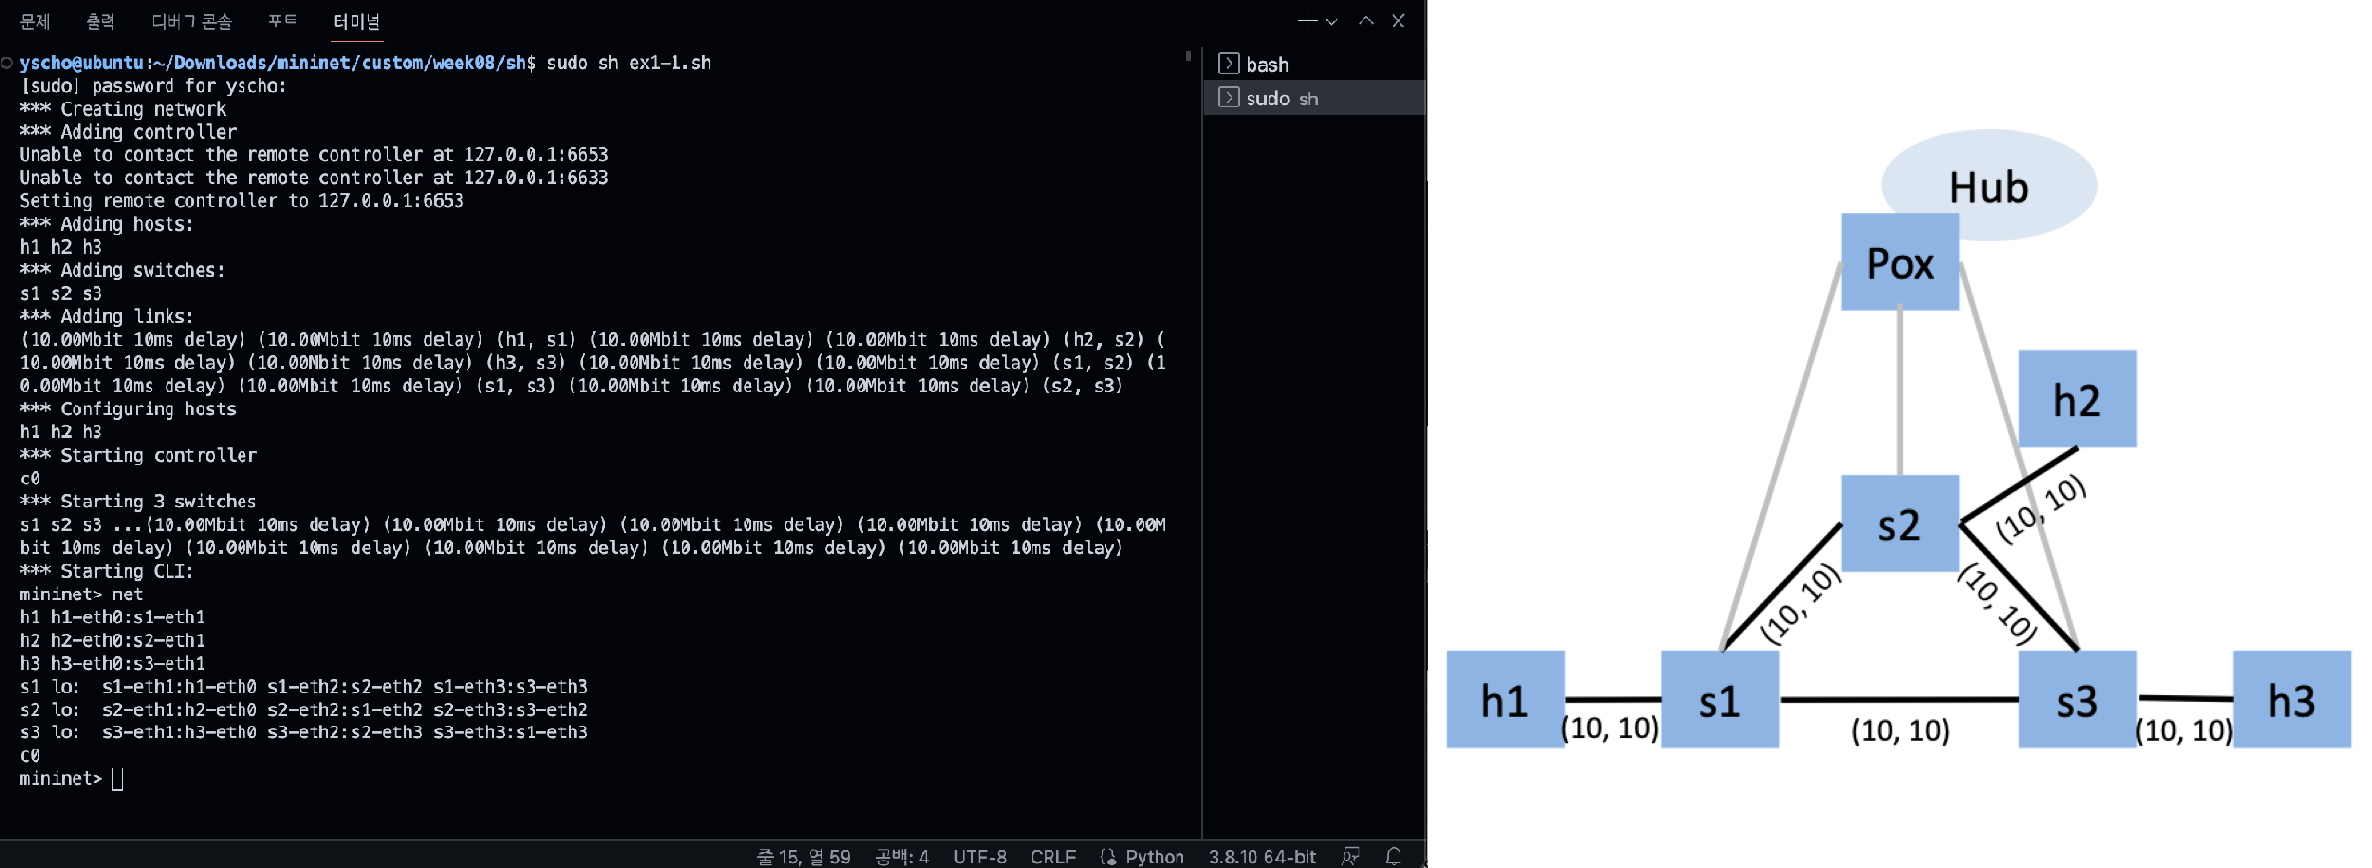
\includegraphics[width=.99\textwidth]{image/week08/1-0.png}
	\caption{\footnotesize
	Ring.py 의 Topology를 실행시킨이후 ,Net command를 이용하여 포트들의 연결을 확인하였다. }
	\vspace{-10pt}
\end{figure}
\clearpage

\subsubsection*{Ping Test}
h1 $\to$ h3의 ping test 결과 switching loop가 발생해서 packet들이 중복수신이 되어, 네트워크에 포화를 일으키는 현상을 발견할 수 있다. \\
\vspace{-4mm}
\begin{figure}[!h]\centering 
	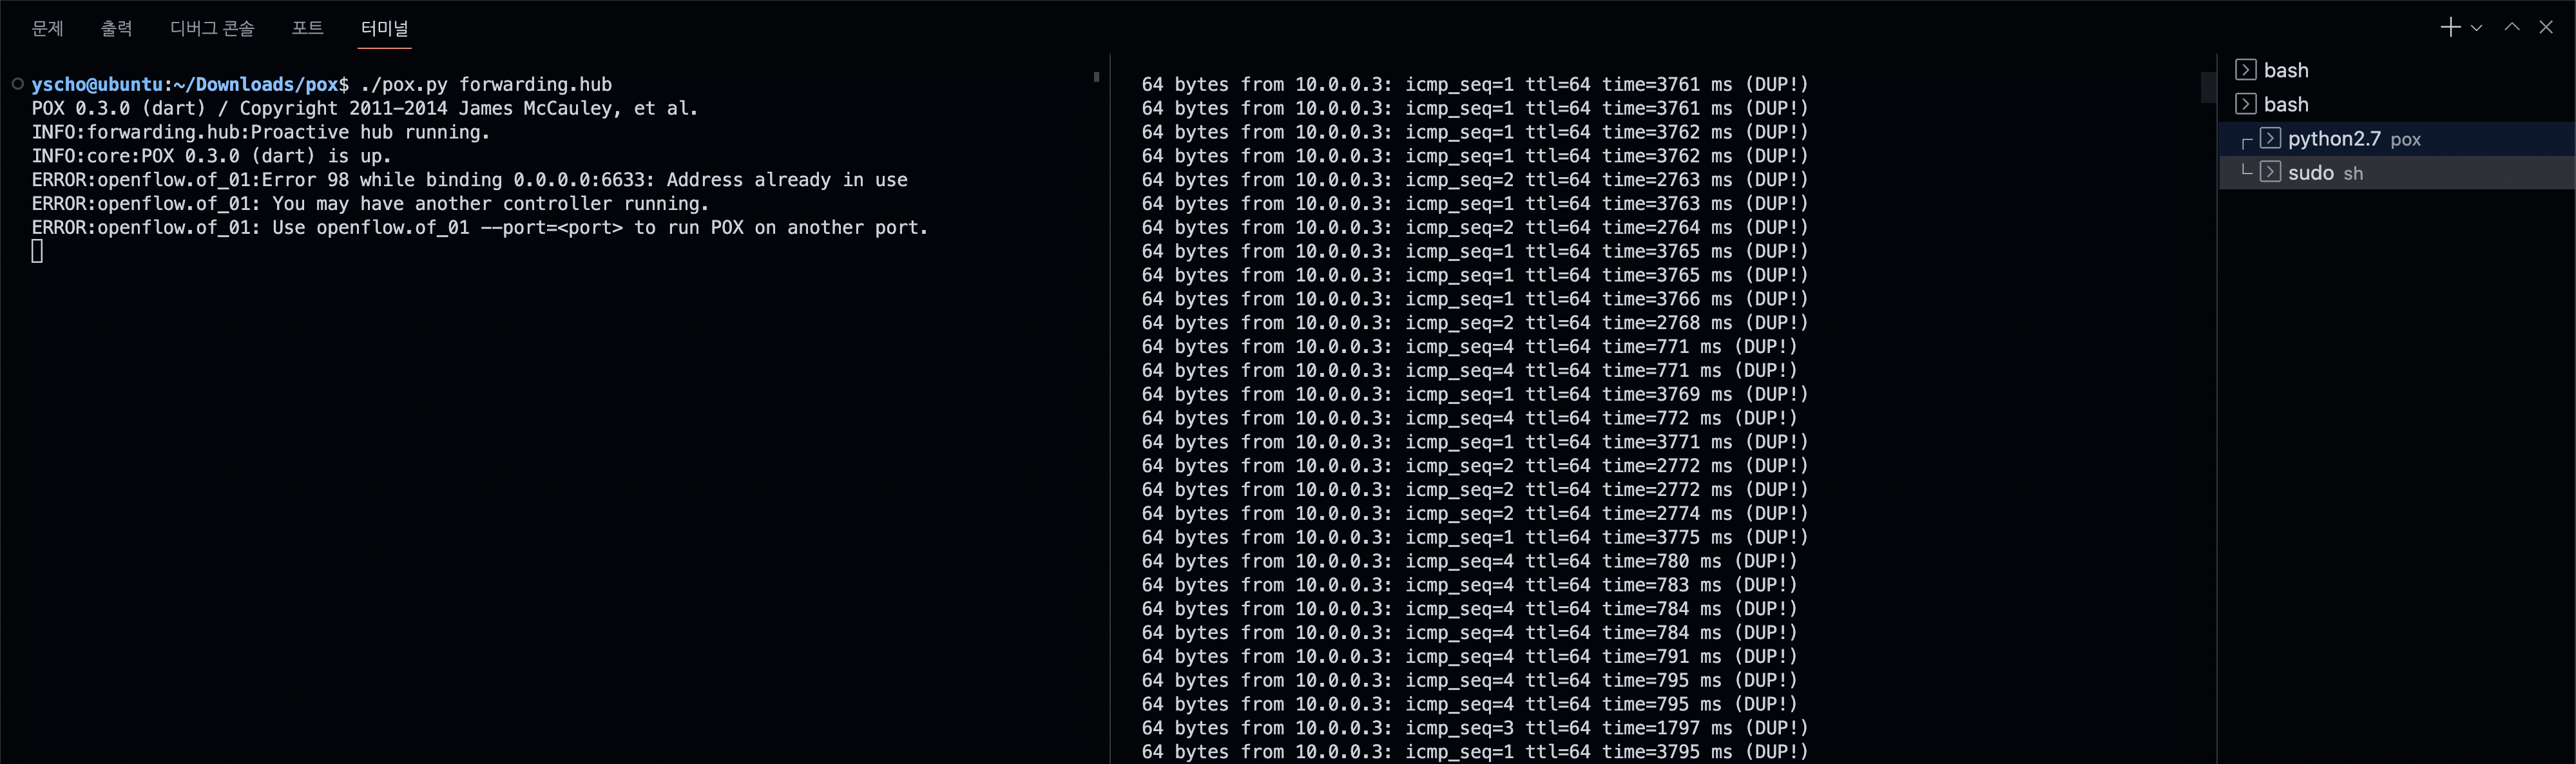
\includegraphics[width=.99\textwidth]{image/week08/1-1.png}
	\caption{\footnotesize
	Switching Loop로 Packet이  중복수신되는것이 확인된다. }
	\vspace{-10pt}
\end{figure}
%%%%%%%%%%%%%%%%%%%%%%%%%%%%%%%%%%%%%%%%%%%%%%%%%%%%%%%%%%%%%%%%%%%%%%%%%%
                        % Experiment 1 - 2
%%%%%%%%%%%%%%%%%%%%%%%%%%%%%%%%%%%%%%%%%%%%%%%%%%%%%%%%%%%%%%%%%%%%%%%%%%
    \vspace{-4mm}
\subsection{Spanning Tree with POX controller }
실험 1-1의 Switching loop가 발생하는 Topology에서 POX controller 를 이용하여 Spannign Tree를 구현해주어 \textit{Switching Loop}를 사라지게하는 실험을 진행한다. POX controller로 discovery.py를 이용하여 controller가 \textbf{LLDP protocol}\footnote{\textbf{Link Layer Discovery Protocol} : LLDP는 LAN에서 시스템이 서로 구성 및 관리 정보를 교환하는 프로토콜이다. 이 정보에는 시스템 기능, 관리 주소 및 기타 네트워크 작업 관련 정보가 포함될 수 있어, LLDP 프로토콜 이용시 시스템이 동일한 로컬 네트워크에 있는 다른 시스템에 대한 유사한 정보를 받을 수 있다.}를 이용하여 전체 Topology를 파악할 수 있게한 다음, spanning\_tree.py 의 알고리즘을 이용해서 파악한 Topology에서 Spanning Tree를 구성한다.

mininet에서 환경을 구성해보고, Tree 구성의 확인과 Ping test결과를 확인하여 STP이 \textit{Switching Loop}를 어떻게 방지하는지 확인해보고자 한다. 
    \vspace{-2mm}
\subsubsection*{Checking Tree's connection with 'dpctl' command}
    \vspace{-2mm}
\begin{figure}[!h]\centering 
	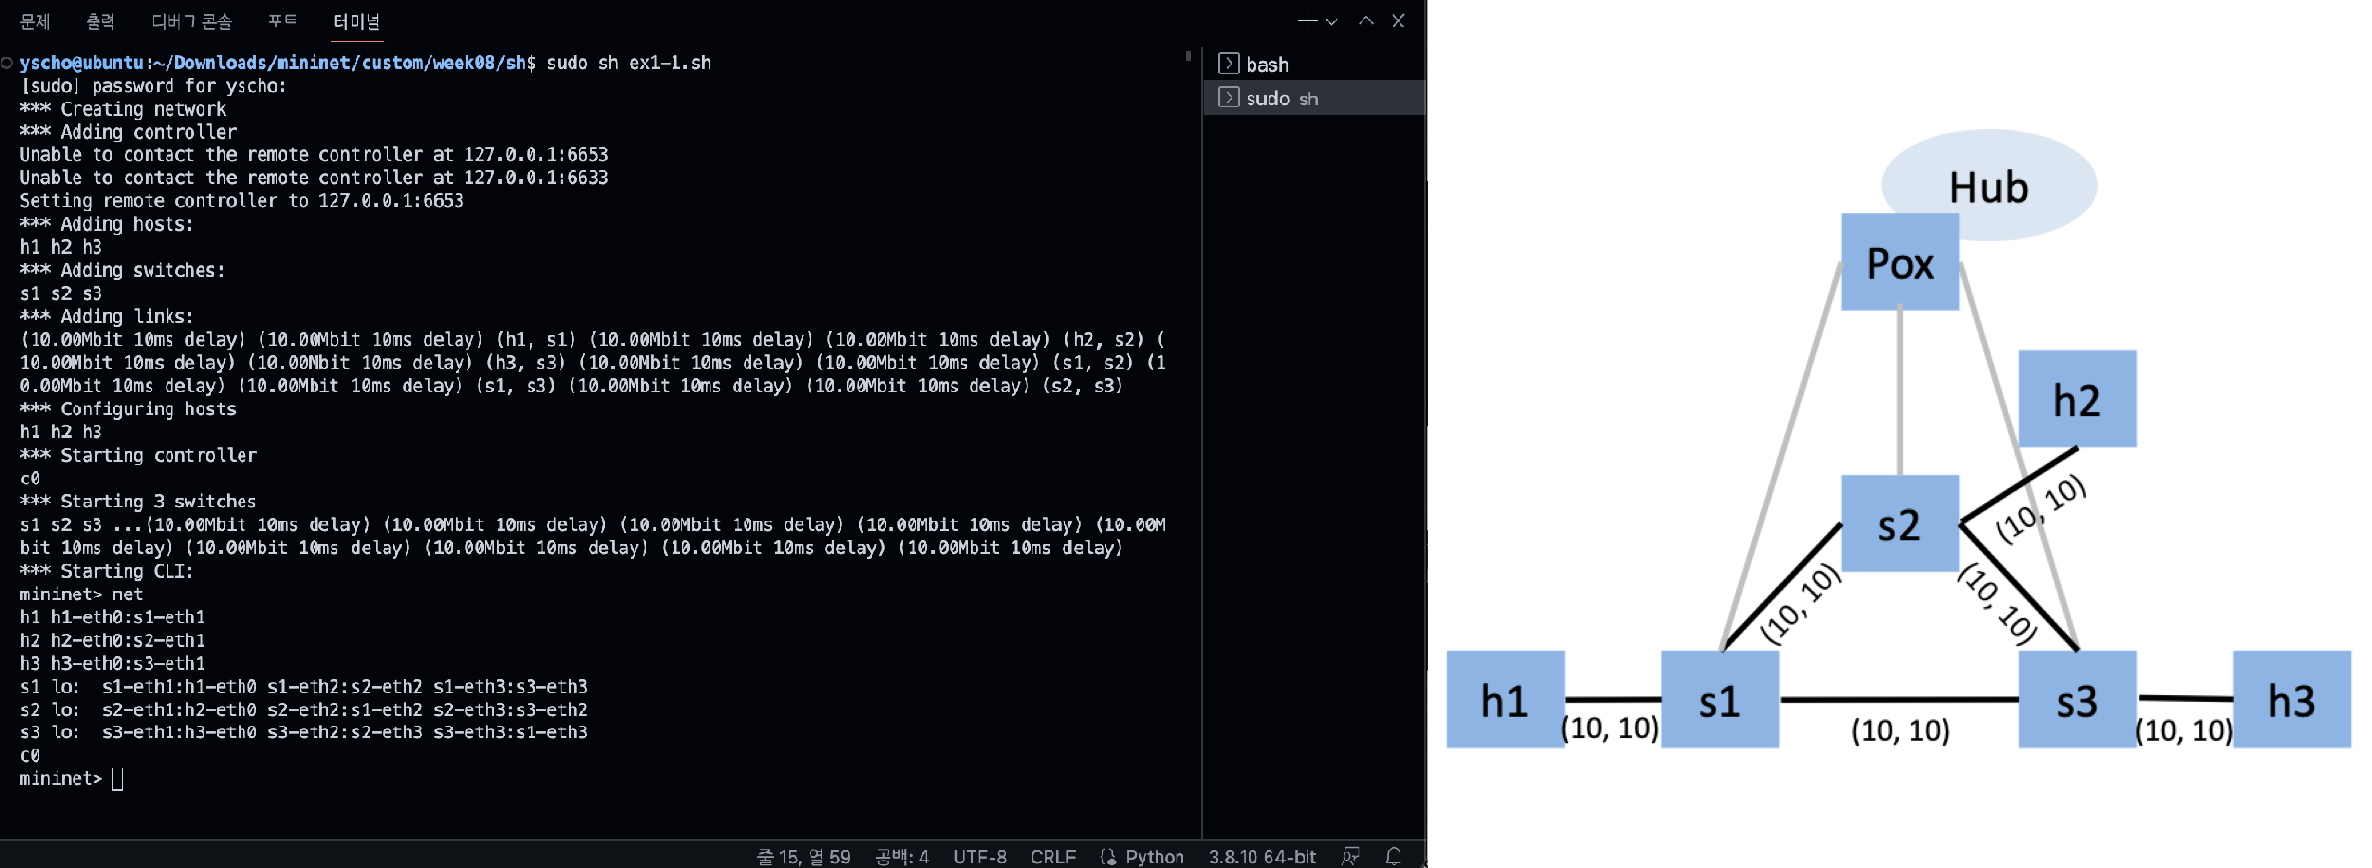
\includegraphics[width=.99\textwidth]{image/week08/1-2-0.png}
	\caption{\footnotesize
	1-1 실험에서 \textit{Switching Loop} 를 일으키는 Network의 Diagram을 다시 확인해보자. }
	\vspace{-10pt}
\end{figure}
1-1에서 \textit{Switching Loop}가 발생되는 network의 diagram과 비교해 보자. dump-ports-desc command를 이용해서 Tree에서 포트간의 연결상태를 확인할 수 있다. Figure 4에서 Controller를 실행시킨 이후 스위치 S2의 3번 포트와 스위치 s3의 2번 포트가 NO\_FLOOD'로 차단되어 있음을 확인할 수 있다.

이제 Ping Test를 통해서 Ping의 도달여부와 Custom Topology를 구성하면서 설정해준 Link 별 10ms의 delay를 통하여 Ping들의 평균 RTT를 확인하여 path를 확인해 \textit{Switching Loop}가 발생하는지 확인해 보자.
\clearpage
\vspace{-4mm}
\begin{figure}[!h]\centering 
	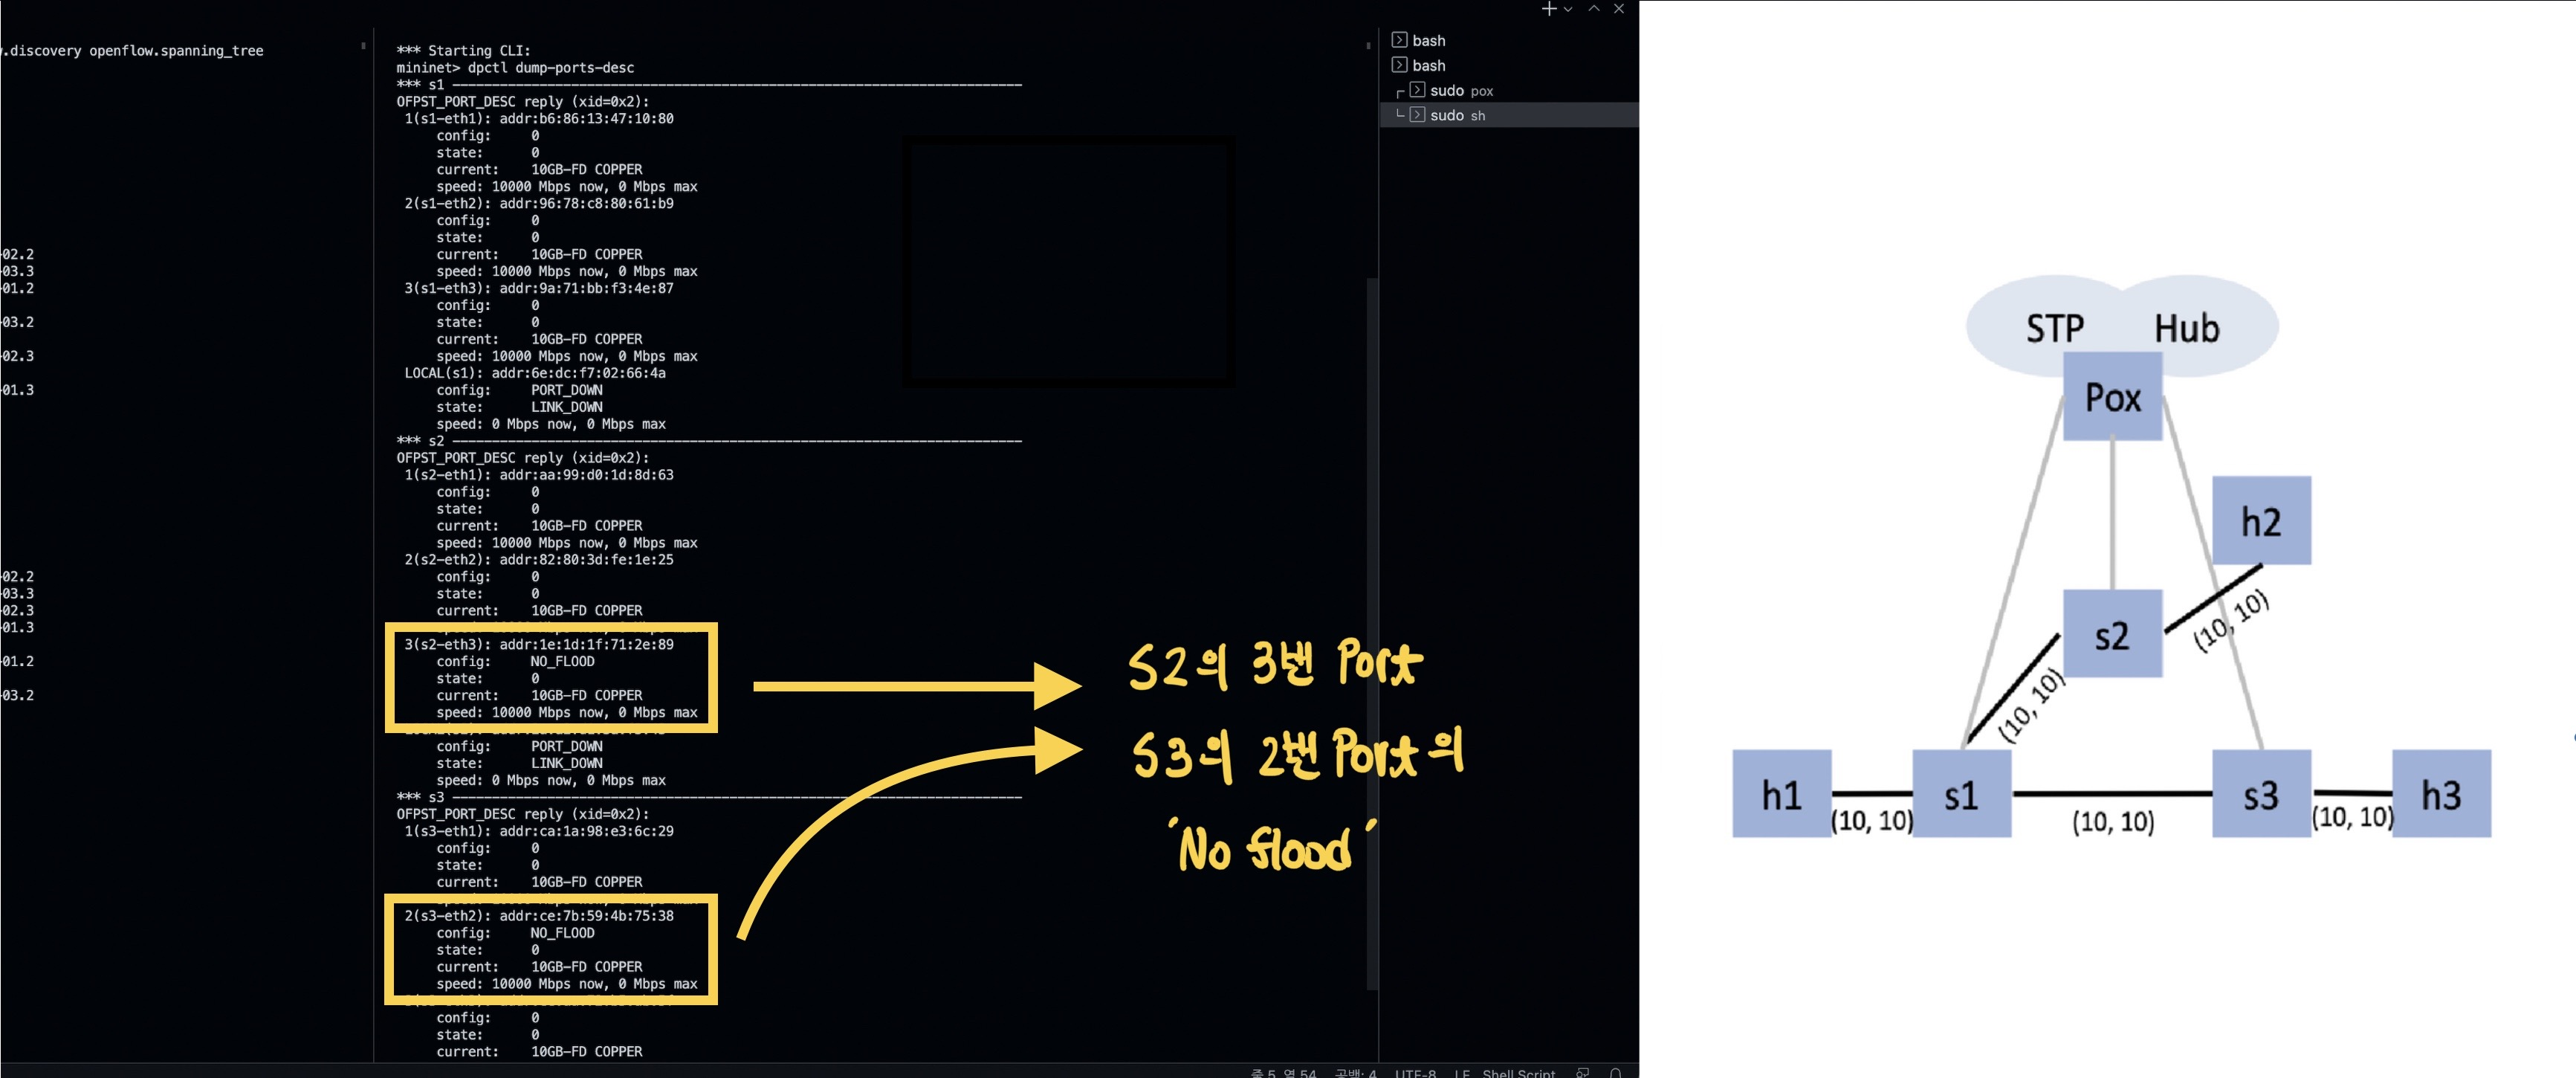
\includegraphics[width=.99\textwidth]{image/week08/1-2-1.png}
	\caption{\footnotesize
	POX Controller의 ~ spanning tree의의 구현을 통해서 특정 S2의 3번 포트 , S3 의 2번 포트가 차단된다.}
	\vspace{-10pt}
\end{figure}
    \vspace{-4mm}
\subsubsection*{Ping Test : h1 $\to$ h3}
\quad h1 $\to$ h2 의 pingtest 결과 Experiment 1-1 과 다르게 Spanning Tree를 구현함으로서, Ping의 전달이 원활히 이루어지는것을 확인할 수 있다. Figrue 1- 2-1의 그림의 경로를 참고하여 총 10ms의  delay를 가지는  link 를 6번 거치므로 Average RTT $\sim$ 60 의 결과를 확인할 수 있다. \\
\vspace{-4mm}
\begin{figure}[!h]\centering 
	\includegraphics[width=.99\textwidth]{image/week08/1-2-2-1.png}
	\caption{\footnotesize
	h1 → h3 with 1000 packet , interval = 0.01   }
	\vspace{-10pt}
\end{figure}
    \vspace{-4mm}
\subsubsection*{Ping Test : h2 $\to$ h3} 
\quad h2 $\to$ h3 pingtest의 결과 또한 마찬가지로 10ms의 delay를 가지는 link를 8번 거치므로 Average RTT $\sim$ 80의 결과를 확인할 수 있다.\\
\vspace{-4mm}
\begin{figure}[!h]\centering 
	\includegraphics[width=.99\textwidth]{image/week08/1-2-2-2.png}
	\caption{\footnotesize
	h1 → h3 with 1000 packet , interval = 0.01  }
	\vspace{-10pt}
\end{figure}
\clearpage
%%%%%%%%%%%%%%%%% need to FIX
